\documentclass[a4paper,12pt]{report}

\usepackage{alltt, fancyvrb, url}
\usepackage{graphicx}
\usepackage[utf8]{inputenc}
\usepackage{float}
\usepackage{hyperref}

% Questo commentalo se vuoi scrivere in inglese.
\usepackage[italian]{babel}

\usepackage[italian]{cleveref}

\title{Relazione per\\``Programmazione ad Oggetti''}

\author{Nicolò Guerra \and
Emma Leonardi \and 
Filippo Casadei \and
Lorenzo Tagliani}
\date{\today}

\begin{document}

\maketitle

\section{Design dettagliato}
\subsection{Lorenzo Tagliani}
\subsubsection{Generazione delle bolle}

\begin{figure}[H]
	\centering{}
	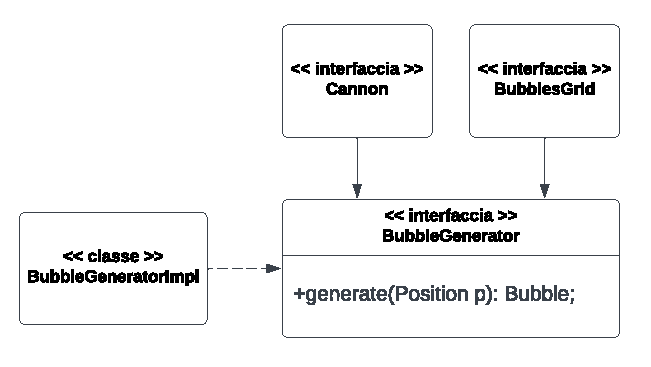
\includegraphics[width=\textwidth]{img/bubblegenerator.pdf}
	\caption{Rappresentazione UML dell'oggetto BubbleGenerator}
\end{figure}

\paragraph{Problema} Nel progetto è stata necessaria, molteplici volte, una generazione casuale delle bolle.

\paragraph{Soluzione} È stato creato un generatore che, basandosi sulla posizione della bolla da posiziona sulla griglia, sfrutta una lista di colori dichiarata per generare una bolla di colore casuale.
Si è preferito fare un generatore come oggetto a se stante invece di implementarlo nel cannone o nella griglia stessa.

\subsubsection{Gestione dei punteggi}

\begin{figure}[H]
	\centering{}
	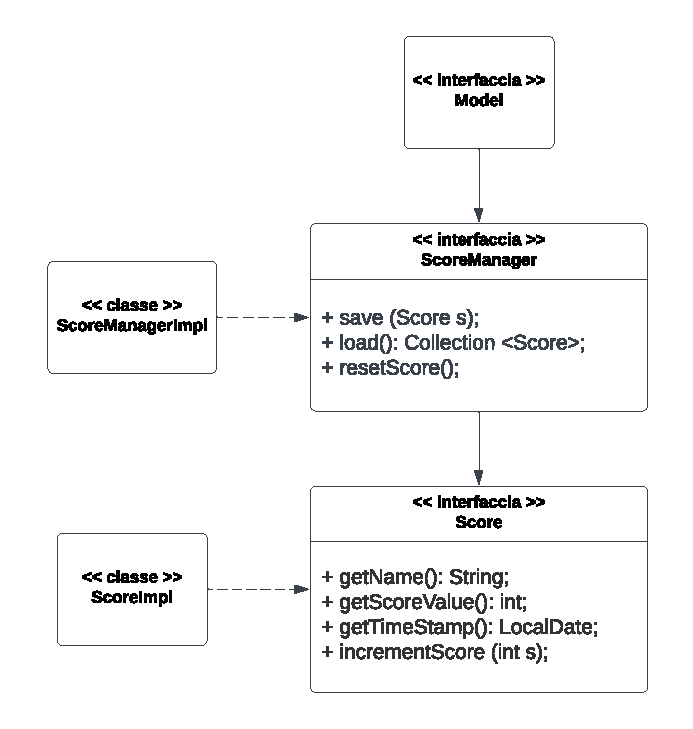
\includegraphics[width=\textwidth]{img/score.pdf}
	\caption{Rappresentazione UML della gestione dei punteggi}
\end{figure}

\paragraph{Problema} Uno degli obiettivi pricipali del progetto era il salvataggio dei punteggi su file, ed al caricamento di essi a richiesta del sistema.

\paragraph{Soluzione} È stato deciso che il punteggio ottenuto dall'utente dovesse essere composto di nome dell'utente, punteggio e data, per questo è stato creato l'oggetto Score, usato poi nello ScoreManager per poter salvare i punteggi su un file, tramite il File Persister creato da Nicolò Guerra.
La lista viene creata e gestita dalla classe ScoreTable, creata per semplificare e organizzare meglio il tutto.

\subsubsection{Gestione della GameView per il giocatore singolo}

\begin{figure}[H]
	\centering{}
	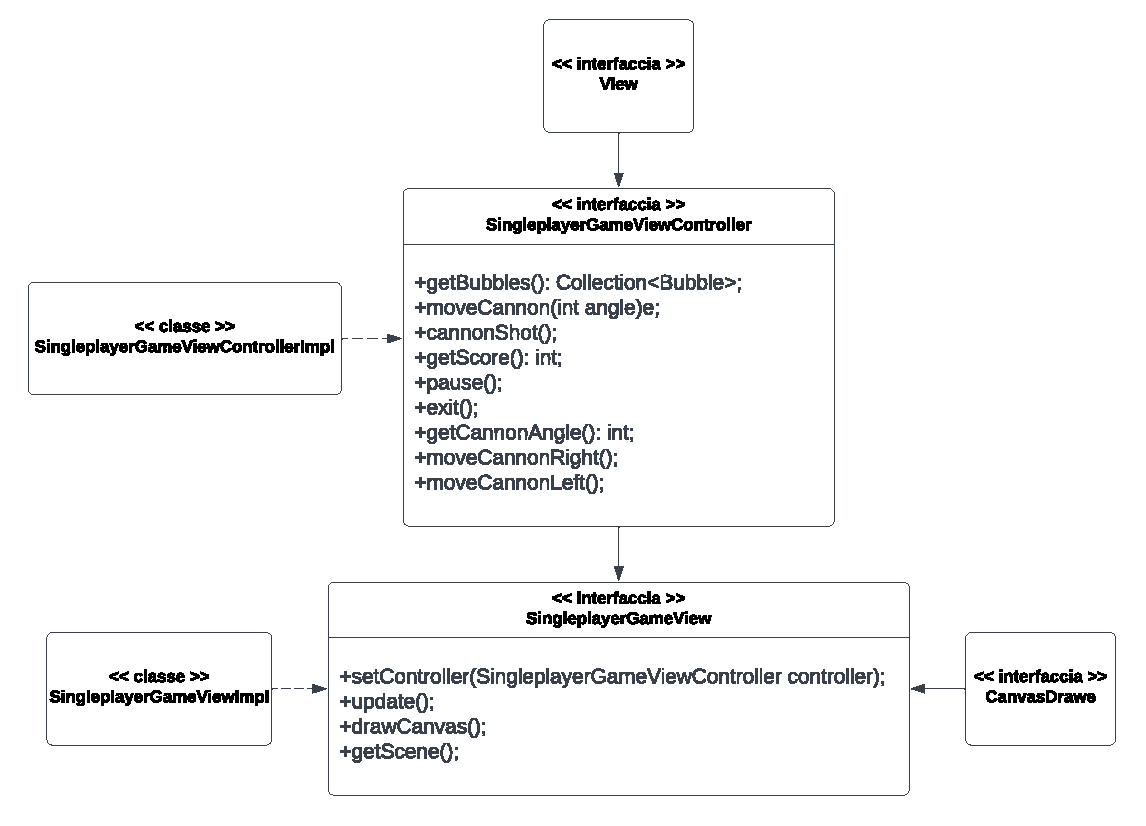
\includegraphics[width=\textwidth]{img/singleplayergameview.pdf}
	\caption{Rappresentazione UML della GameView singleplayer}
\end{figure}

\paragraph{Problema} Per il giocatore singolo era necessaria una GameView organizzativa.

\paragraph{Soluzione} 

\end{document}